%-----------------------------------------------------------------------------
%
%               Template for sigplanconf LaTeX Class
%
% Name:         sigplanconf-template.tex
%
% Purpose:      A template for sigplanconf.cls, which is a LaTeX 2e class
%               file for SIGPLAN conference proceedings.
%
% Guide:        Refer to "Author's Guide to the ACM SIGPLAN Class,"
%               sigplanconf-guide.pdf
%
% Author:       Paul C. Anagnostopoulos
%               Windfall Software
%               978 371-2316
%               paul@windfall.com
%
% Created:      15 February 2005
%
%-----------------------------------------------------------------------------


\documentclass[10pt, reprint]{sigplanconf}

% The following \documentclass options may be useful:

% preprint      Remove this option only once the paper is in final form.
% 10pt          To set in 10-point type instead of 9-point.
% 11pt          To set in 11-point type instead of 9-point.
% authoryear    To obtain author/year citation style instead of numeric.

\usepackage{amsmath}
\usepackage{graphicx}
\usepackage[space]{grffile}
\usepackage{latexsym}
\usepackage{amsfonts,amsmath,amssymb}
\usepackage{url}
\usepackage[utf8]{inputenc}
\usepackage{hyperref}
\hypersetup{colorlinks=false,pdfborder={0 0 0}}
\usepackage{textcomp}
\usepackage{longtable}
\usepackage{multirow,booktabs}
\usepackage{enumitem}
\usepackage{adjustbox}
\usepackage{balance}

%%%%%%%%
\usepackage[firstpage]{draftwatermark}
\SetWatermarkText{\textsc{Confidential}}
\SetWatermarkScale{1.2}
\SetWatermarkColor[gray]{0.9}
\SetWatermarkFontSize{2cm}
\SetWatermarkAngle{45}
%%%%%%%%

\newcommand{\noauthorea}{}
\input{header}

\begin{document}

\special{papersize=8.5in,11in}
\setlength{\pdfpageheight}{\paperheight}
\setlength{\pdfpagewidth}{\paperwidth}

\conferenceinfo{CONF 'yy}{Month d--d, 20yy, City, ST, Country} 
\copyrightyear{2015} 
\copyrightdata{978-1-nnnn-nnnn-n/yy/mm} 
\doi{nnnnnnn.nnnnnnn}

% Uncomment one of the following two, if you are not going for the 
% traditional copyright transfer agreement.

%\exclusivelicense                % ACM gets exclusive license to publish, 
                                  % you retain copyright

%\permissiontopublish             % ACM gets nonexclusive license to publish
                                  % (paid open-access papers, 
                                  % short abstracts)

\titlebanner{banner above paper title}        % These are ignored unless
\preprintfooter{short description of paper}   % 'preprint' option specified.

\newcommand{\anon}{$\bullet\bullet\bullet\bullet\bullet$}

\title{Platform Agnostic On-Stack Replacement in LLVM
  
  }
%\subtitle{Subtitle Text, if any}

\iffalse
\authorinfo{\anon\ \and \anon}
           {\anon} % affil
           {\anon} % email
\fi

\authorinfo{Daniele Cono D'Elia \and Camil Demetrescu}
           {{\small Dept. of Computer, Control, and Management Engineering\\Sapienza University of Rome}} % affil
           {\{demetres,delia\}@dis.uniroma1.it} % email

\maketitle

\begin{abstract}
% !TEX root = article.tex

On-Stack Replacement (OSR) is a technique for dynamically transferring execution between different versions of a function at run time.
%suspending the execution of a function and continuing with a different version of the code. 
OSR is often used in virtual machines to interrupt a long-running function and recompile it at a higher optimization level, or to replace it with a different one when a speculative assumption made during its compilation no longer holds.

In this paper we present a framework for OSR that introduces novel ideas and combines features of extant techniques that no previous solution provided simultaneously. New features include OSR with compensation code to adjust the program state during a transition and the ability to fire an OSR from arbitrary locations in the code. Our approach is platform-independent as the OSR machinery is entirely encoded at a compiler's intermediate representation level.

%Compared to extant OSR techniques, our approach is platform-independent as transitions are encoded entirely at the Intermediate Representation (IR) level; it supports OSR-point insertion at arbitrary locations in a function, 

%and it allows a function version reached via OSR to fire an OSR itself, either to a more optimized version or to a less optimized one from which it was derived.

We implement and evaluate our technique in the LLVM compiler infrastructure, which is nowadays being increasingly used as Just-In-Time (JIT) compiler in virtual machines for dynamic languages such as Javascript, MATLAB, Python, and Ruby. We also present a case study on the integration of our technique in the McVM virtual machine for MATLAB, showing significant speedups from the run-time optimization of a typical construct of the language.
  
  
  
  
  
  
  
  
  
\end{abstract}

\category{D.3}{Processors}{Compilers}

% general terms are not compulsory anymore, 
% you may leave them out
%\terms
%term1, term2

\keywords
On-stack replacement, just-in-time compilation, code optimization, deoptimization, LLVM.

\cite{fink2003design}\section{Introduction}
\label{se:intro}

[...]

  
  
  
  
% !TEX root = article.tex

\ifdefined\noauthorea
\begin{figure}[t]
\begin{center}
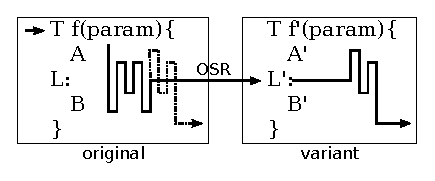
\includegraphics[width=0.6\columnwidth]{figures/overview-osr/overview-osr.eps}
\caption{\protect\label{fig:osr-dynamics} On-stack replacement dynamics
  
  
  }
\end{center}
\end{figure}
\fi

\section{Overview}
\label{se:overview}

In this section we provide an overview of the approach we propose. The key to platform independence in our work is to express the entire OSR machinery at intermediate code representation level, without resorting to machine-level code manipulation or special intrinsics of the intermediate language such as Stackmap and Patchpoint in LLVM IR. %Before describing how this is achieved in LLVM, we provide an overview of our approach.

%\subsection{Overview}
%\label{ss:overview}

Consider the generic OSR scenario shown in \myfigure\ref{fi:osr-dynamics}. A base function \fbase\ is executed and it can either terminate normally (dashed lines), or an OSR event may transfer control to a variant \fvariant, which resumes the execution. The decision of whether an OSR should be fired at a given point \osrpoint\ of \fbase\ is based on an {\em OSR condition}. A typical example in JIT-based virtual machines is a profile counter reaching a certain hotness threshold, which indicates that \fbase\ is taking longer than expected and is worth optimizing. Another example is a guard testing whether \fbase\ has become unsafe and execution needs to fall back to a safe version \fvariant. This scenario includes deoptimization of functions generated with aggressive speculative optimizations. 

Several OSR implementations adjust the stack so that execution can continue in \fvariant\ with the current frame \cite{chambers1991self,holzle1992self, suganuma2006region}. This requires manipulating the program state at machine-code level and is highly ABI- and compiler-dependent. A simpler approach, which we follow in this article, consists in creating a new frame every time an OSR is fired, essentially regarding an OSR transition as a function call~\cite{lameed2013modular,webkit14}. 

Our implementation targets two general scenarios: 1) {\em resolved OSR}: \fvariant\ is known before executing \fbase\ as in the deoptimization example discussed above; 2) {\em open OSR}: \fvariant\ is generated when the OSR is fired, supporting deferred and profile-guided compilation strategies. In both cases, \fbase\ is instrumented before its execution to incorporate the OSR machinery. We call such OSR-instrumented version \fosrfrom.

In the resolved OSR scenario (see \myfigure\ref{fi:overview-osr-final}), instrumentation consists of adding a check of the OSR condition and, if it is satisfied, a tail call that fires the OSR. The called function is an instrumented version of \fvariant, which we call \fosrto. We refer to \fosrto\ as the {\em continuation function} for an OSR transition. The assumption is that \fosrto\ produces the same side-effects and return value that one would obtain by \fbase\ if no OSR was performed. Differently from \fvariant, \fosrto\ takes as input all live variables of \fbase\ at \osrpoint, executes an optional compensation code to fix the computation state ({\tt comp\_code}), and then jumps to a point \textsf{L'} from which execution can continue. The OSR practice often makes the conservative assumption that execution can always continue with the very same program state as the base function. However, this assumption may reduce the number of
%safe
points where OSR transitions can be fired. Supporting compensation code in our framework adds flexibility, allowing OSR transitions to happen at arbitrary places in the base function.

\ifdefined\noauthorea
\begin{figure}[t]
\begin{center}
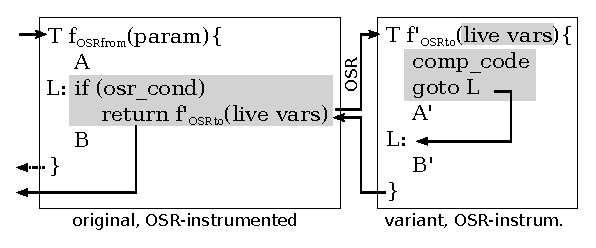
\includegraphics[width=0.7\columnwidth]{figures/overview-osr-final/overview-osr-final.eps}
\caption{\protect\label{fi:overview-osr-final} OSR-instrumented functions.
  
  }
\end{center}
\end{figure}
\fi

\ifdefined\noauthorea
\begin{figure}[h!]
\begin{center}
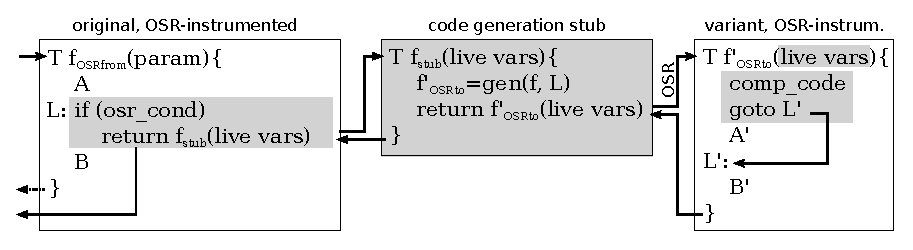
\includegraphics[width=1.0\columnwidth]{figures/overview-osr-open/overview-osr-open.eps}
\caption{\protect\label{fi:overview-osr-open} Open OSR scenario. Instrumentation code is in grey.
  
  
  
  
  }
\end{center}
\end{figure}
\fi

\noindent The open OSR scenario is similar, with one main difference (see \myfigure\ref{fi:overview-osr-open}): instead of calling \fosrto\ directly, \fosrfrom\ calls a stub function \fstub, which first creates \fosrto\ and then calls it. Function \fosrto\ is generated by a function {\tt gen} that takes the base function \fbase\ and the OSR point \osrpoint\ as input. The reason for having a stub in the open OSR scenario, rather than directly instrumenting \fbase\ with the code generation machinery, is to minimize the extra code injected into \fbase. Indeed, instrumentation may interfere with optimizations, e.g., by increasing register pressure and altering code layout and instruction cache behavior.


\paragraph{Discussion.}
Instrumenting functions for OSR at a higher level than machine code yields several benefits: 
\begin{enumerate}
\item {\em Platform independence}: the OSR instrumentation code is lowered to native code by the compiler back-end, which handles the details of the target ABI. 
\item {\em Global optimizations}: lowering OSR instrumentation code along with application code can generate faster code than local binary instrumentation. For instance, dead code elimination can suppress from \fosrto\ portions of code that would no longer be needed when jumping to the landing pad \textsf{L'}, producing smaller code and enabling better register allocation and instruction scheduling.
\item {\em Debugging and Profiling}: preserving ABI conventions in the native code versions of \fosrfrom, \fstub, and \fosrto\ helps debuggers and profilers to more precisely locate the current execution context and collect more informative data.
%avoiding low-lever tampering with stack frames can more easily preserve ABI calling conventions
\item {\em Abstraction}: being entirely encoded using high-level language constructs (assignments, conditionals, function calls), the approach is amenable to a clean instrumentation API that abstracts the OSR implementation details, allowing a front-end to focus on where to insert OSR points independently of the final target architecture.
%by analyzing code at an intermediate representation level.
\end{enumerate}

\noindent A natural question is whether encoding OSR at a higher level of abstraction can result in poorer performance than binary code approaches. We address this issue in \mysection\ref{se:osr-llvm}, where we analyze the OSR machine code generated for an x86-64 target, and in \mysection\ref{se:experiments}, where OSR performance is measured on classic benchmarks.

\section{OSR in LLVM}
\label{se:osr-llvm}

In this section we discuss our implementation of the approach described in \ref{se:overview} in \tinyvm, a proof-of-concept virtual machine we developed as a playground to exercise our OSR techniques. TinyVM is based on LLVM's MCJIT compiler and supports interactive invocation of LLVM IR functions either generated at run-time or loaded from disk. The main design goal behind TinyVM is the creation of an interactive environment for IR manipulation and JIT-compilation of functions: for instance, it allows the user to insert OSR points in loaded functions, run optimization passes on them or display their CFGs, repeatedly invoke a function for a specified amount of times and so on. TinyVM supports dynamic library loading and linking, and comes with a helper component for MCJIT that simplifies tasks such as handling multiple IR modules, symbol resolution in presence of multiple versions of a function, and tracking native code and other machine-level generated object such as Stackmaps.

To explain how \tinyvm\ works, we consider the running example of \myfigure\ref{fi:isord-example}.

\ifdefined\noauthorea
\begin{figure}[t]
\begin{center}

\includegraphics[width=0.9\columnwidth]{figures/isord-example/isord.eps}
\caption{\protect\label{fi:isord-example} Example for OSR instrumentation in LLVM.
}
\end{center}
\end{figure}
\fi

\ifdefined\noauthorea
\begin{figure}[t]
\begin{center}
\includegraphics[width=0.9\columnwidth]{figures/isordfrom/isordfrom.eps}
\caption{\protect\label{fig:isordfrom} LLVM IR version of base function {\tt isord} (\myfigure\ref{fi:isord-example}) instrumented for open OSR. The OSR is fired at the beginning of the loop body after 1000 iterations. Additions resulting from the instrumentation are in grey.
}
\end{center}
\end{figure}
\fi

\ifdefined\noauthorea
\begin{figure}[t]
\begin{center}
\includegraphics[width=0.9\columnwidth]{figures/isordascto/isordascto.eps}
\caption{\protect\label{fig:isordascto} LLVM IR version of faster, specialized variant of {\tt isord} (\myfigure\ref{fi:isord-example}) instrumented for OSR. Instrumentation additions are in grey. The original function entry block is unreachable after instrumentation and is eliminated (struck-through code fragments).}
\end{center}
\end{figure}
\fi

\ifdefined\noauthorea
\begin{figure}[t]
\begin{center}
\includegraphics[width=0.9\columnwidth]{figures/isordx86-64/isordx86-64.eps}
\caption{\protect\label{fig:isordx86-64} OSR-instrumented functions {\tt isordfrom} (base) and {\tt isordascto} (faster continuation) after IR to x86-64 lowering in LLVM. Additions resulting from the IR instrumentation are in grey, while removals are struck-through.}
\end{center}
\end{figure}
\fi

\subsection{Resolved OSR Points}

\subsection{Open OSR Points}
  
%\begin{verbatim}
%int fac(int n) {
%    int i = 2, f = 1;
%    while (i<=n) f *= i++;
%    return f;
%}
%\end{verbatim}
%
%\begin{verbatim}
%int fac(int n) {
%    int i = 2, f = 1;
%    while (i<=n)  {
%        if (osr_cond) return fac_osr(n,i,f); 
%        f *= i++; 
%    } return f;
%}
%\end{verbatim}
%
%\begin{verbatim}
%int fac_osr(int n) {
%    goto L;
%    int i = 2, f = 1;
%    while (i<=n) L: f *= i++;
%    return f;
%}
%\end{verbatim}


  
  
  
  
  
\section{Case Study}
\label{case-study}

MATLAB is a popular dynamic language for scientific and numerical programming. Introduced in the late 1970s mainly as a scripting language for performing computations through efficient libraries, it has evolved over the years into a more complex programming language with support for high-level features such as functions, packages and object orientation. A popular feature of the language is the {\tt feval} construct, a built-in higher-order function that enable the invocation of the function passed as first argument on the set of subsequent arguments of the {\tt feval} call, and to return the computed result. This feature is heavily used in many classes of numerical computations, such as iterative methods for the approximation of the solutions of ordinary differential equations and simulated annealing heuristics to locate a good approximation to the global optimum of a function in a large search space.

A previous study by Lameed and Hendren~\cite{lameed2013feval} shows that the overhead of an {\tt feval} call is significantly high compared to a direct call, especially in JIT-based execution environments such as McVM and the proprietary MATLAB JIT accelerator by Mathworks. The main reason for this overhead is that the presence of an {\tt feval} instruction can disrupt the results of intra- and inter-procedural level for type and array shape inference analyses, which are a key ingredient for efficient code generation.

Lameed and Hendren thus propose and implement in McVM two dynamic techniques for optimizing {\tt feval} instructions. The first technique is based on OSR: using the McOSR library~\cite{lameed2013modular}, {\tt feval} calls inside loops are instrumented with an OSR point and with profiling code to cache the last-known types for the arguments of each {\tt feval} instruction. When an OSR is fired at run-time, a code generator modifies the original function by inserting a guard to choose between a fast path containing a direct call and a slow path with the original {\tt feval} call. The second technique is less general and uses value-based JIT compilation: when the first argument of an {\tt feval} call is an argument of the enclosing function, the compiler replaces each call to this function in all of its callers with a call to a special dispatcher. When the program is executed, the dispatcher will evaluate the value of the parameter for the {\tt feval} and execute either a previously compiled cached code or generate and JIT-compile a method optimized for the current value of the argument.

Although the OSR-based approach is more general, it generates much less efficient code compared to the JIT-based version for three reasons:
\begin{enumerate}
\item since the function called through {\tt feval} is unknown at compile time, the type inference engine is unable to infer types for the returned values, so the compiler has to generate generic instructions (suitable for handling different types) for the remainder of the code;
\item guard computation is expensive, because not only the value of the first argument, but also the types of the remaining arguments have to be checked to choose between the fast and the slow path;
\item since an {\tt feval} is executed through the interpreter, in the original functions arguments are boxed to make them more generic before the call.
\end{enumerate}

The first one in particular is a major source of inefficiency for the OSR-based approach, since the benefits from replacing the call to the interpreter's {\tt feval} dispatcher with a direct call are limited compared to the optimization opportunities deriving from a better type inference on the whole body of the function. In fact, as they operate on boxed values, instructions operating on generic-type variables are inherently much less efficient than their counterparts for [arrays of] primitive types. While the JIT-based approach is preferable as it generates much better code, on the other hand it cannot be applied to cases in which the first argument $f$ to {\tt feval} is not passed as argument to the enclosing function $g$. Some possible scenarios are:
\begin{itemize}
\item $f$ is an {\tt inline} or an anonymous function defined in $g$;
\item $f$ is the return value from a previous call in $g$ to another function;
%\item $f$ is retrieved from a data structure~\cite{lameed2013feval};
\item $f$ is a constant string containing the name of a user-defined function (a typical inappropriate use of {\tt feval} according to~\cite{radpour2013refactoring}).
\end{itemize}
 
Lameed and Hendren conclude their paper by stating, ``It would be interesting to look at future work that combine the
strengths of both approaches". In the remaining part of this section, we extend McVM by implementing a novel optimization mechanism for {\tt feval} based on our OSR technique: we will show that our mechanism is as efficient as their JIT-based approach in terms of quality of generated code, and is even more general than their OSR-based approach, as it can optimize also {\tt feval} calls not enclosed in a loop.

\subsection{Extending McVM}
The McVM virtual machine is a complex research project developed at McGill and composed of several software components, including: a front-end for lowering MATLAB programs to an intermediate representation called IIR that captures all of the high-level features of the language; an interpreter for running MATLAB functions and scripts in IIR format; a manager component to perform analyses on IIR; a JIT compiler based on LLVM for generating native code for a function, thus lowering McVM IIR to LLVM IR; a set of helper components to perform fast vector and matrix operations using optimized libraries such as ATLAS, BLAS and LAPACK. The architecture of McVM is illustrated in Figure [...]

McVM implements a JIT specialization mechanism for functions based on call signatures: for each IIR representation of a function, multiple IR versions are generated according to the types of the arguments for the call




  
  
  
  
% !TEX root = article.tex

\subsection{Comparison to previous approaches}
\label{ss:prev-eval-sol}

Lameed and Hendren~\cite{lameed2013feval} proposed two dynamic techniques for optimizing \feval\ instructions in McVM: {\em OSR-based} and {\em JIT-based} specialization, which work as follows.

\paragraph{JIT-based specialization.}  

[...]

\paragraph{OSR-based specialization.} When a loop containing an \feval\ becomes hot in a function $f$, an OSR is triggered. At that time, an optimized version $f'$ of $f$ is generated and control is diverted to $f'$. $f'$ is created by an optimizer that attempts to replace an \feval$(g,x,y,z...)$ instruction with a direct call $g(x,y,z,...)$ with unboxed parameters. The optimizer uses the actual values of $g$ and its arguments known at the OSR time to specialize the code. The direct call is guarded by a condition that checks if $g$ and the type of its parameters remain the same as observed when the OSR was fired. If the guard fails, the code falls back to executing the original \feval\ instruction.

While this method overcomes the limitations of JIT-based specialization, supporting optimization of \feval\ instructions without , it is substantially slower for two main reasons:
\begin{enumerate}
\item when a function $f$ is first compiled from MATLAB to IR by McVM, the functions it calls via \feval\ are unknown. Hence, the type inference engine is unable to infer types for their returned values, and these values must be kept boxed in heap-allocated objects and handled with slow generic instructions in the IR representation of $f$ (suitable for handling different types). For this reason, the optimized continuation functions $f'$ generated at OSR points in McVM inherit the slow generic instructions of $f$.
\item guard computation in $f'$ can be rather expensive, as it may require checking many parameters;
\end{enumerate}

\noindent Our approach combines the flexibility of OSR-based specialization with the efficiency of JIT-based specialization, answering an open question raised by Lameed and Hendren~\cite{lameed2013feval}. Indeed, [...]

{\tt [Daniele --> text moved from case-study.tex]} Compared to the OSR-based approach by Lameed and Hendren, our solution is cheaper because the types for the other arguments do not need to be cached or guarded: as we will see later on, the type inference engine will compute the most accurate yet sound type information in the analysis of the optimized IIR where direct calls are used.

\ifdefined\fullver
The first one is based on OSR: using the McOSR library~\cite{lameed2013modular}, \feval\ calls inside loops are instrumented with an OSR point and profiling code to cache the last-known types for the arguments of each \feval\ instruction. When an OSR is fired at run-time, a code generator modifies the original function by inserting a guard to choose between a fast path containing a direct call and a slow path with the original \feval\ call. The second technique is less general and uses value-based JIT compilation: when the first argument of an \feval\ call is an argument of the enclosing function, the compiler replaces each call to this function in all of its callers with a call to a special dispatcher. At run-time, the dispatcher evaluates the value of the argument to use for the \feval\ and executes either a previously compiled cached code or generates and JIT-compiles a version of the function optimized for the current value.

Although the OSR-based approach is more general, it generates much less efficient code compared to the JIT-based one for three reasons:
\begin{enumerate}
\item since the function called through \feval\ is unknown at compile time, the type inference engine is unable to infer types for the returned values, so the compiler has to generate generic instructions (suitable for handling different types) for the remainder of the code;
\item guard computation is expensive, not only because the value of the first argument, but also the types of the remaining arguments have to be checked to choose between the fast and the slow path;
\item since an \feval\ is executed through the interpreter, arguments are boxed to make them more generic before the call.
\end{enumerate}

The first one in particular is a major source of inefficiency for the OSR-based approach, since the benefits from replacing the call to the interpreter's \feval\ dispatcher with a direct call are limited compared to the optimization opportunities deriving from a better type inference on the whole body of the function. In fact, as they operate on boxed values, instructions for generic-type variables are inherently much less efficient than their counterparts for [arrays of] primitive types. While the JIT-based approach is preferable as it generates much better code, on the other hand it cannot be applied to cases in which the first argument $f$ to \feval\ is not passed as argument to the enclosing function $g$. Some possible scenarios for MATLAB programs are:
\begin{itemize}
\item $f$ is an {\tt inline} or an anonymous function defined in $g$;
\item $f$ is the return value from a previous call in $g$ to another function;
%\item $f$ is retrieved from a data structure~\cite{lameed2013feval};
\item $f$ is a constant string containing the name of a user-defined function (a typical misuse of \feval ~\cite{radpour2013refactoring}).
\end{itemize}
 
Lameed and Hendren conclude their paper by stating, ``It would be interesting to look at future work that combine the
strengths of both approaches". In the remaining part of this section, we extend McVM by implementing a novel optimization mechanism for \feval\ based on our OSR technique: we will show that our mechanism is as efficient as their JIT-based approach in terms of quality of generated code, and is even more general than their OSR-based approach, as it can optimize also \feval\ calls not enclosed in a loop.
\fi


% !TEX root = article.tex

\subsection{A New Approach}
\label{ss:eval-opt-mcvm}

In this section, we present a new approach that combines the flexibility of OSR-based specialization with the efficiency of the JIT-based method, answering an open question raised by Lameed and Hendren~\cite{lameed2013feval}. The key idea is to lift the $f$-to-$f'$ optimization performed by the OSR-based specialization from IR to IIR level. This makes it possible to perform type inference in $f'$, generating a much more efficient code. The main technical challenge of this idea is that the program's state in $f$ at the OSR point may be incompatible with the state of $f'$ from which execution continues. Indeed, some variables may be boxed in $f$ and unboxed in $f'$. Hence, compensation code is needed to adjust the state by performing live variable unboxing during the OSR.

%The main idea for optimizing a function $f$ containing an \feval\ instruction is to dynamically generate a variant $f'$ where the \feval$(g,...)$ is replaced by a direct call of the form $g(...)$. The key to efficiency is the ability to perform type inference on the IIR level, [...]

%capture run-time information

\paragraph{Implementation in McVM.}
We implemented our approach in McVM\footnote{As a by-product of our project, we ported the MATLAB McVM virtual machine from the LLVM legacy JIT to the new MCJIT toolkit.}, extending it with four main components:

\ifdefined \noauthorea
\begin{enumerate}[noitemsep]
\else
\begin{enumerate}
\fi
\item An analysis pass to identify optimization opportunities for \feval\ instructions in the IIR of a function.
\item An extension for the IIR compiler to track the mapping between IIR and IR objects at \feval\ sites.
\item An OSR inserter based on \osrkit\ to inject open OSR points in the IR for IIR locations annotated during the analysis pass.
\item An \feval\ optimizer triggered at OSR points, which uses:
\ifdefined \noauthorea
\begin{enumerate}[noitemsep]
\else
\begin{enumerate}
\fi
\item a profile-driven IIR generator to replace \feval\ calls with direct calls;
\item a helper component to lower the optimized IIR function to IR and construct a state mapping;
\item a code caching mechanism to handle the compilation of the continuation functions.
\end{enumerate}
\end{enumerate}

\noindent We remark that our implementation heavily depends on \osrkit's ability to handle compensation code. 

\ifdefined \fullver
\paragraph{Analysis Pass.} The analysis pass, which is fully integrated in McVM's analysis manager, groups \feval\ instructions whose first argument is reached by the same definition, and for each group marks for instrumentation only those instructions not dominated by others, so that the function can be optimized as early as possible at run-time. 
\ifdefined \fullver
It is also able to determine whether the value of the argument can change across two executions of the same \feval\ instruction, thus discriminating when a run-time guard must be inserted during the run-time optimization phase.
\else
It also determines whether the value of the argument can change across two executions of the same \feval, and a run-time guard must thus be inserted during the optimization phase.
\fi

\paragraph{IIR Compiler Extension.}
The extension operates when the IIR compiler processes an annotated \feval\ instruction. It builds a {\em variable map} between IIR and IR objects, and keeps track of the {\tt llvm::BasicBlock*} $b$ created for the \feval\  in the IR code and of the {\tt llvm::Value*} object $g$ used as its first argument. 

\paragraph{OSR Inserter.}
The OSR inserter uses the $b$ and $g$ objects collected by the compiler extension as basic block and {\tt val} argument in the open-OSR stub that invokes the \feval\ optimizer, respectively.
\fi

%The last two elements are then used by the inserter component as basic block and {\tt val} argument in the open-OSR stub that invokes the optimizer component.

\newcommand{\gBase}{$f$}
\newcommand{\gOpt}{$f_{opt}$}
\newcommand{\gIIR}{$f^{IIR}$}
\newcommand{\gIR}{$f^{IR}$}
\newcommand{\gOptIIR}{$f^{IIR}_{opt}$}
\newcommand{\gOptIR}{$f^{IR}_{opt}$}

%%%%%%%%%%%%%%%%%%%%%%%%%%%%%
\paragraph{Optimizer.}
The core of our optimization pipeline is the optimizer module, which is responsible for generating optimized code for the running function \gBase\ using contextual information passed by an open-OSR stub. As a first step, the optimizer inspects {\tt val} to resolve the target $f$ of the \feval\ and checks whether a previously compiled version of \gBase\ optimized for $f$ is available from the cache.
\ifdefined \fullver
If not, a new function \gOpt\ is generated by cloning the IIR representation \gIIR\ of \gBase\ into \gOptIIR\ and replacing all the \feval\ calls in the same group of the instrumented one with direct calls to $f$.
\else
If not, a new function \gOpt\ is generated by cloning the IIR representation \gIIR\ of \gBase\ into \gOptIIR\ and replacing all \feval\ calls to $f$ with direct calls.
\fi

As a next step, the optimizer asks the IIR compiler to process \gOptIIR\ and generate optimized LLVM IR \gOptIR, also storing the variable map between IIR and IR objects when compiling the direct call corresponding to the \feval\ instruction that triggered the OSR.
\ifdefined \fullver

\fi
This map is essential for the next step, which is constructing a state mapping between \gIR\ to \gOptIR, as it is compared against the corresponding map stored during the lowering of \gBase\ to determine whether for each value in \gOptIR\ live at the continuation block:
\begin{itemize}
\item an {\tt llvm::Value*} from \gIR\ passed as argument at the OSR point can be used directly
\item or, compensation code is required to reconstruct its value before jumping to the block.
\end{itemize}

\noindent In fact, since the type inference engine yields more accurate results for \gOptIIR\ compared to \gIIR, the IIR compiler can in turn generate efficient specialized IR code for representing and manipulating IIR variables, and compensation code is typically required to unbox or downcast some of the live values passed at the OSR point.
\ifdefined \fullver
Compensation code might also be required to materialize an IR object for an IIR variable that were previously accessed through get/set methods from the environment. %TODO
\fi

Once a state mapping object has been constructed, the optimizer calls our OSR library to generate the continuation function for the OSR transition and eventually compiles it. A pointer to the compiled function is stored in the code cache and returned to the stub, which invokes it through an indirect call passing the live state saved at the OSR point.

%%%%%%%%%%%%%%%%%%%%%%%%%%%%%
\paragraph{Discussion.}
The ideas presented in this section advance the state of the art of \feval\ optimization in MATLAB runtimes.
%combine the flexibility of OSR-based specialization with the efficiency of the JIT-based method. 
Similarly to OSR-based specialization, we do not place restrictions on the functions that can be optimized. On the other hand, we work at IIR (rather than IR) level as in JIT-based specialization, which allows us to perform type inference on the specialized code. Working at IIR level eliminates the two main sources of inefficiency of OSR-based specialization: 1) we can replace generic istructions with specialized instructions, and 2) the types of $g$'s arguments do not need to be cached or guarded as they are statically inferred. These observations are confirmed in practice by experiments on benchmarks from the MATLAB community, as we will show in \mysection\ref{ss:experim-results}.

\section{Experimental Evaluation}
\label{se:experiments}

In this section we present a preliminar experimental study of our OSR technique in TinyVM, a proof-of-concept virtual machine based on LLVM's JIT compiler MCJIT. TinyVM supports interactive invocations of functions and it can compile LLVM IR either generated at run-time or loaded from disk. The main design goal behind TinyVM is the creation of an interactive environment for IR manipulation and JIT-compilation of functions: for instance, it allows the user to insert OSR points in loaded functions, run optimization passes on them or display their CFGs, repeatedly invoke a function for a specified amount of times and so on. TinyVM supports dynamic library loading and linking, and comes with a helper component for MCJIT that simplifies tasks such as handling multiple IR modules, symbol resolution in presence of multiple versions of a function, and tracking native code and other machine-level generated object such as Stackmaps.

TinyVM is thus an ideal playground to exercise our OSR technique, and we use it to run performance measurements on the shootout test suite, also known as the Computer Language Benchmark Game~\cite{shootout}. The list of benchmarks and their description is reported in Table~\ref{tab:shootout}; four of them - namely {\tt b-trees}, {\tt mbrot}, {\tt n-body} and {\tt sp-norm} - are evaluated against two workloads of different size.

\begin{table} 
    \begin{tabular}{ |c|c| }
        \hline
        {\em Benchmark} & {\em Description} \\ 
        \hline
        \hline
        b-trees & Adaptation of a GC bench for binary trees \\ 
        \hline
        fannkuch & Fannkuch benchmark on permutations \\ 
        \hline
        fasta & Generation of DNA sequences \\ 
        \hline
        fasta-redux & Generation of DNA sequences (with lookup table) \\ 
        \hline
        mbrot & Mandelbrot set generation \\ 
        \hline
        n-body & N-body simulation of Jovian planets \\ 
        \hline
        rev-comp & Reverse-complement of DNA sequences \\ 
        \hline
        sp-norm & Eigenvalue calculation with power method \\ 
        \hline
    \end{tabular} 
    \caption{\label{tab:shootout} Description of the shootout benchmarks} 
\end{table}

\subsection{Setup}

We generated the IR modules for our experiments with clang, starting from the C version of the shootout suite. No LLVM optimization passes were performed on the code other than {\em mem2reg}, which promotes memory references to be register references and is typically used in SSA form construction.

Experiments were performed on an octa-core 2.3 Ghz Intel Xeon E5-4610 v2 with 256+256KB of L1 cache, 2MB of L2 cache, 16MB of shared L3 cache and 128 GB of DDR3 main memory, running Debian Wheezy 7, Linux kernel 3.2.0, LLVM 3.6.2 (Release build, compiled using gcc 4.7.2), 64 bit.

For each benchmark we performed 10 trials preceded by an initial warm-up iteration; reported confidence intervals are stated at 95\% confidence level.

\subsection{Results}

\begin{itemize}
\item {\bf Message 1}: how much does a never-firing OSR point impact code quality? We run a program with one or more OSR points, and we measure the slowdown given by factors such as cache effects (due to code bloat), register pressure, etc. due to the presence of the OSR points.
\item {\bf Message 2}: what is the overhead of an OSR transition to the same function? We run a program with a controlled OSR transition, e.g., with a counter that fires the OSR. Here we measure the impact of the actual OSR call [we already tried this with the repeated addition microbenchmark simple\_loop\_SSA.ll].
\item {\bf Message 3}: what is the overhead of the library for inserting OSR points? We compute: 1) the average time per OSR transition; 2) the number of transferred live variables; 3) the total benchmark time with an always-firing OSR at each iteration of the hottest loop; 4) the total benchmark time without OSR instrumentation (baseline).
\end{itemize}

\paragraph{Impact on code quality}
In order to measure how much a never-firing OSR point might impact code quality, we analyzed the source-code structure of each benchmark and profiled its run-time behavior to identify performance-critical sections for OSR point insertion.

For iterative benchmarks, we insert an OSR point in the body of their hottest loops. We classify a loop as hottest when its body is executed for a very high cumulative number of iterations (e.g., from a few thousands up to billions) and it either calls the method with the highest {\em self} time in the program, or it performs the most computational-intensive operations for the program in its own body. These loops are natural candidates for OSR point insertion, as they can be used - as in the Jikes RVM - to enable more dynamic inlining opportunities, with the benefits from several control-flow (e.g., dead code elimination) and data-flow (e.g., constant propagation) optimizations based on the run-time values of the live variables. In the shootout benchmarks, the number of such loops is typically 1 (2 for {\tt spectral-norm}).

For {\tt b-trees} - the only benchmark in our suite showing a recursive pattern - we insert an OSR point in the body of the method that accounts for the largest {\em self} execution time of the program. Such an OSR point might be useful to trigger recompilation of the code at a higher degree of optimization, or to enable some form of dynamic optimization (for instance, in a recursive search algorithm we might want to inline the comparator method provided by the user at the call).
  
\section{Related Work}
\label{se:related}

\paragraph{Early Approaches.}
%OSR has been pioneered in the SELF language~\cite{holzle1992self} to enable source-level debugging of optimized code, which required deoptimizing the code back to the original version. To reconstruct the source-level state, the compiler generates {\em scope descriptors} recording for each scope the locations or values of its arguments and locals. Execution can be interrupted only at certain interrupt points (i.e., method prologues and backward branches in loops) where its state is guaranteed to be consistent, allowing optimizations between interrupt points. It is worth mentioning also the {\em deferred compilation} mechanism~\cite{chambers1991self} implemented in SELF for branches that are unlikely to occur at run-time: the system generates a stub which invokes the compiler to generate a code object that can reuse the stack frame of the original code.

OSR has been pioneered in the SELF language~\cite{holzle1992self} to enable source-level debugging of optimized code, which required deoptimizing the code back to the original version. To reconstruct the source-level state, the compiler generates {\em scope descriptors} recording locations or values of arguments and locals. Execution can be interrupted only at certain interrupt points where its state is guaranteed to be consistent (i.e., method prologues and backward branches in loops), allowing optimizations between interrupt points. SELF also implements a deferred compilation mechanism~\cite{chambers1991self} for branches that are unlikely to occur at run-time: the system generates a stub which invokes the compiler to generate a code object that can reuse the stack frame of the original code.

\paragraph{Java Virtual Machines.}
The success of the Java language has drawn more attention to the design and implementation of OSR techniques, as bytecode interpreters began to work along with JIT compilers. In the high-performance HotSpot Server JVM~\cite{paleczny2001hotspot} performance-critical methods are identified using method-entry and backward-branches counters; when the OSR threshold is reached, the runtime transfers the execution from the interpreter frame to an OSR frame and the compiled code. Deoptimization is performed when class loading invalidates inlining or other optimization decisions: execution is rolled forward to a safe point, at which the native frame is converted into an interpreter frame.

\ifdefined \fullver
Whaley~\cite{whaley2001osr} proposes a technique to identify intra-method code regions that are rarely executed, and thus compile and optimize the code without these regions. A rare block is replaced by a stub that transfers the control to the interpreter, while a glue routine reconstructs the state from the interpreter starting from a table storing the location, in registers or memory, of each variable in the original bytecode.
\fi

The Jikes RVM uses an OSR mechanism~\cite{fink2003design} that extracts a scope descriptor from a thread suspended at a method's entrypoint or backward branch, creates specialized code to setup the stack frame for the optimized compiled code and resumes the execution at the desired program counter. OSR is used as part of an automatic, online, profile-driven deferred compilation mechanism. A more general approach has then been proposed in~\cite{soman2006efficient}, with the OSR implementation decoupled from program code to ease more aggressive specializations triggered by events external to the executing code (e.g. class loading, exception conditions). Execution state information is maintained in a variable map - a per-method list of thread-switch points and associated live bytecode variables - that is incrementally updated across a wide range of basic compiler optimizations.

\ifdefined \fullver
In the Graal VM - a modified version of HotSpot centered on the principle of speculative optimizations - the execution falls back to the interpreter during deoptimization, while a runtime function restores the stack frames in the interpreter using the metadata associated with the deoptimization point~\cite{duboscq2013graal,wurthinger2013truffle,duboscq2014metadata}.
\else
In the Graal VM, which is centered on speculative optimizations, the execution falls back to the interpreter during deoptimization, while a runtime function restores the stack frames in the interpreter using the metadata associated with the deoptimization point~\cite{duboscq2013graal,wurthinger2013truffle,duboscq2014metadata}.
\fi

% TODO only if we have space: HotpathVM

\paragraph{Prospect.} Prospect~\cite{susskraut2010prospect} is an LLVM-based framework for parallelizing a sequential application. The IR is instrumented through two LLVM passes to enable switching at run-time between a slow and a fast variant of the code, which are both compiled statically. Helper methods are used to save and eventually restore registers, while stack-local variables are put on a separate {\tt alloca} stack rather than on the stack frame so that the two variants result into similar and thus interchangeable stack layouts.
\ifdefined \fullver
Speculative variables~\cite{susskraut2009speculation} are introduced when the slow variant needs to track state (e.g., information for out-of-bound checks) that is missing in the fast variant. Switching operations are performed by Prospect at user-specified checkpoints in the original code.
\fi

\paragraph{McOSR.} McOSR~\cite{lameed2013modular} is a library for the LLVM legacy JIT compiler to insert OSR points at loop headers. When an OSR transition is fired, the live state is saved into a set of global variables (one per live variable) and a helper method is invoked to modify the IR of the function using a code transformer provided by the front-end and a copy of the original code saved as control version. The library generates a new entrypoint for the function to check a global condition and discriminate whether the function is being invoked through an OSR transition or a regular call: in the first case, values for live variables are read from the associated global variables, and the execution jumps to the block to resume the execution at.
\ifdefined \fullver
The SSAUpdater component of LLVM is then used to restore the SSA form after the update.
\fi
When the helper method returns, the updated function is invoked and the OSR is thus performed in a new stack frame. When the updated function returns, a second helper method is called to recompile the updated function to remove the new entrypoint inserted for the OSR transition, as it can disrupt LLVM optimizations and lead to poorer performance on subsequent invocations of the function.

\paragraph{Other Related Work.}
\ifdefined \fullver
Dynamic Software Updating (DSU) is a methodology for permitting programs to be updated while they run and is thus useful for systems that cannot afford to halt service. DSU techniques (e.g. ~\cite{neamtiu2006dsu,makris2009dsu}) are required to update all functions active on the call stack at the same time, so their code should be instrumented and data types wrapped to support future extensions.

\fi
In tracing JIT compilers deoptimization techniques are used to safely leave an optimized trace when a guard fails and to continue the execution in the interpreter or with a different piece of code. SPUR~\cite{bebenita2010spur} is a trace-based JIT compiler for Microsoft's Common Intermediate Language (CIL) with four levels of JIT-ting: profiling, tracing, optimizing and transfer-tail; transfer-tail JIT is used to bridge the execution from an instruction in a block from tracing or optimizing mode to the next safe point for deoptimization to profiling code. In RPython guards are implemented as a conditional jump to a trampoline that analyzes resume information for the guard and executes compensation code to leave the trace. Resume data is compactly encoded by sharing parts of the data structure between subsequent guards~\cite{schneider2012rpython}; a similar approach is used in LuaJIT, where sparse snapshots are taken to enable state restoration when leaving a trace~\cite{luajit}.

% TODO: speculative parallelization? (e.g. FastTrack)

%\cite{detlefs2001method,steiner2007adaptive,chambers1992design}
 % !TEX root = article.tex

\section{Conclusions}
\label{se:conclusions}

In this paper, we have proposed an OSR framework that combines the advantages of different previous OSR techniques that no previous solution provides simultaneously.


%, without resorting to native code manipulation or special instrinsics of the intermediate level.
Our solution combines in a unifying framework the advantages of different previous OSR techniques that no previous solution provides simultaneously.


scheme for encoding OSR machinery using high-level language constructs. 

%our continuation function is specialized for a given OSR landing pad and allows extensive optimizations.

\ifx\noauthorea\undefined
\paragraph{Acknowledgements.}

We wish to thank Jan Vitek, Petr Maj, Karl Millar, and Olivier Fl{\"u}ckiger for many enlightening discussions. We are especially grateful to Jan for sparking our interest in this exciting line of research. % during a pleasant visit at Purdue University and for interesting conversations in many other occasions.
\fi

% !TEX root = ../article.tex

% LaTeX template for Artifact Evaluation V20151015
%
% Prepared by Grigori Fursin (cTuning foundation, France and dividiti, UK) 
% and Bruce Childers (University of Pittsburgh, USA)
%
% (C)opyright 2014-2015


%%%%%%%%%%%%%%%%%%%%%%%%%%%%%%%%%%%%%%%%%%%%%%%%%%%%
% When adding this appendix to your paper, 
% please remove above part
%%%%%%%%%%%%%%%%%%%%%%%%%%%%%%%%%%%%%%%%%%%%%%%%%%%%

\appendix
\section{Artifact Description}

%\newcommand{\nomcvm}{}

%Submission and reviewing guidelines and methodology: \\
%{\em http://cTuning.org/ae/submission-20151015.html}

%%%%%%%%%%%%%%%%%%%%%%%%%%%%%%%%%%%%%%%%%%%%%%%%%%%%%%%%%%%%%%%%%%%%%
\subsection{Abstract}

\osrkit\ is a library that enables On-Stack Replacement (OSR) at arbitrary places in LLVM IR code. The artifact is designed to explore how \osrkit\ can instrument IR code to support OSR transitions in the LLVM MCJIT runtime environment. A running example is presented based on the \texttt{isord} case study discussed in Section 3. We also support repeating all the experiments presented in Section 5. The artifact includes an interactive VM called \tinyvm\ for loading, inspecting, instrumenting, and executing IR code. The package is a preconfigured Oracle VirtualBox VM.


%%%%%%%%%%%%%%%%%%%%%%%%%%%%%%%%%%%%%%%%%%%%%%%%%%%%%%%%%%%%%%%%%%%%%
\subsection{Description}

The main component of the artifact is an interactive VM called \tinyvm\ built on top of the LLVM MCJIT runtime environment and the \osrkit\ library. The VM provides an interactive environment for IR manipulation, JIT-compilation, and execution of functions either generated at run-time or loaded from disk: for instance, it allows the user to insert OSR points in loaded functions, run optimization passes on them, display their CFGs, and repeatedly invoke a function for a specified amount of times. \tinyvm\ supports dynamic library loading and linking, and includes a helper component for MCJIT that simplifies tasks such as handling multiple IR modules, symbol resolution in presence of multiple versions of a function, and tracking machine-level generated code and data objects.

\tinyvm\ is located in {\small\tt /home/osrkit/Desktop/tinyvm/} and runs a case-insensitive command-line interpreter:
\begin{small}
\begin{verbatim}
osrkit@osrkit-AE:~/Desktop/tinyvm$ tinyvm
Welcome! Enter 'HELP' to show the list of commands.
TinyVM> 
\end{verbatim}
\end{small}

\noindent Use {\tt HELP} to print basic documentation on how to use the shell. Usage scenarios are discussed in \ref{ss:art-eval-res}.

\subsubsection{Check-list (artifact meta information)}

%{\em Fill in whatever is applicable with some informal keywords and remove the rest}

{\small
\begin{itemize}[parsep=0pt]
  %\item {\bf Algorithm: }
  \item {\bf Program: } {\tt shootout} C benchmarks (included, Sep 2015). %and a number of MATLAB benchmarks (included)
  \item {\bf Compilation: } LLVM 3.6.2 (release build).
  %\item {\bf Transformations: }
  %\item {\bf Binary: }
  %\item {\bf Data set: }
  \item {\bf Run-time environment: } Linux (version 3.x).
  \item {\bf Hardware: } x86-64 CPU.
  \item {\bf Run-time state: } Cache-sensitive (performance measurements only).
  %\item {\bf Execution: }
  \item {\bf Output: } Measures are output to console.
  \item {\bf Experiment workflow: } Invoke scripts and perform a few manual steps.
  \item {\bf Publicly available?} Yes.
\end{itemize}
}

\subsubsection{How Delivered}

The artifact ships as an Oracle VirtualBox 5 Appliance.
The latest version of the code is available at \url{https://github.com/dcdelia/tinyvm}.

\subsubsection{Hardware Dependencies}

An x86-64 platform is required.

\subsubsection{Software Dependencies}

The artifact was tested in Oracle VirtualBox 5.0.10. 

%\subsubsection{Datasets}

%%%%%%%%%%%%%%%%%%%%%%%%%%%%%%%%%%%%%%%%%%%%%%%%%%%%%%%%%%%%%%%%%%%%%
\subsection{Installation}

To install the artifact, just import the appliance in Oracle VirtualBox, which installs Linux LXLE. Open the {\tt README} file on the {\tt Desktop} folder for further info on the artifact and the Linux distribution.

%%%%%%%%%%%%%%%%%%%%%%%%%%%%%%%%%%%%%%%%%%%%%%%%%%%%%%%%%%%%%%%%%%%%%
\subsection{Experiment Workflow}

\ifdefined \nomcvm
We propose two usage sessions. In the first session, we show how to generate and instrument an LLVM IR code based on the \texttt{isord} example presented in \mysection\ref{se:osr-llvm}. The second session focuses on how to run the scripts used to generate the performance tables of \mysection\ref{se:experiments} related to questions Q1, Q2, and Q3. Question Q4 is based on additional third-party software (the MATLAB McVM runtime\footnote{The source code of the version used in the paper, which we ported to LLVM 3.6+ and extended with the {\tt feval} optimization technique discussed in \ref{ss:eval-opt-mcvm}, is available at \url{https://github.com/dcdelia/mcvm}.}) and is not addressed in the artifact.
\else
We propose three usage sessions. In the first session, we show how to generate and instrument an LLVM IR code based on the \texttt{isord} example presented in \mysection\ref{se:osr-llvm}. The second session focuses on how to run the scripts used to generate the performance tables of \mysection\ref{se:experiments} related to questions Q1, Q2, and Q3. The third session addresses question Q4, using third-party software (the MATLAB McVM runtime~\cite{mcvm}) that we ported to LLVM 3.6+ and extended with the {\tt feval} optimization technique discussed in \ref{ss:eval-opt-mcvm}.
\fi

%%%%%%%%%%%%%%%%%%%%%%%%%%%%%%%%%%%%%%%%%%%%%%%%%%%%%%%%%%%%%%%%%%%%%
\subsection{Evaluation and Expected Result}
\label{ss:art-eval-res}

% !TEX root = ../article.tex

\subsubsection{Session 1: OSR instrumentation in \osrkit}

\tinyvm\ implements a code generator for open OSR points that can dynamically inline function calls to targets that cannot be statically determined. In the example from \myfigure\ref{fi:isord-example}, a comparator function {\tt c} is passed as argument to function {\tt isord}, which checks whether an array {\tt v} of numbers is ordered according to the criterion encoded in {\tt c}.

To interactively reproduce the experiment presented in \mysection\ref{se:osr-llvm}, we provide under the folder {\small\tt tinyvm/isord} a C module {\small\tt inline.c} with an LLVM IR counterpart {\small\tt inline.ll} (generated with {\small\tt clang -S -emit-llvm -O1 inline.c}).

\vspace{0.2em}
We can load the IR module in \tinyvm\ and show the code generated for method {\tt isord} with:
\begin{small}
\begin{verbatim}
osrkit@osrkit-AE:~/Desktop/tinyvm$ tinyvm
Welcome! Enter 'HELP' to show the list of commands.
TinyVM> LOAD_IR isord/inline.ll
[LOAD] Opening "isord/inline.ll" as IR source file...
TinyVM> DUMP isord
[...]
\end{verbatim}
\end{small}

\noindent Displayed virtual register names and basic block labels will often differ from those reported in \myfigure\ref{fig:isordfrom}, which have been refactored for the sake of readability. In particular, the loop body of {\tt isord} will look like:

\begin{small}
\begin{verbatim}
.lr.ph:                          ; preds = %2, %0
  %i.01 = phi i64 [ %10, %2 ], [ 1, %0 ]
  %4 = getelementptr inbounds i64* %v, i64 %i.01
  %.sum = add nsw i64 %i.01, -1
  %5 = getelementptr inbounds i64* %v, i64 %.sum
  %6 = bitcast i64* %5 to i8*
  %7 = bitcast i64* %4 to i8*
  %8 = tail call i32 %c(i8* %6, i8* %7) #3
  [...]
\end{verbatim}
\end{small}

\noindent A $\phi$-node {\tt \%i.01} is used to represent the index of the {\tt for} loop from the C code, and is set to {\tt \%10} when reached from the loop header (basic block {\tt \%2}) {\em after} a loop iteration. In fact, as a result of {\small \tt -O1} optimizations, when {\tt n>1} execution jumps from the function entrypoint {\tt \%0} directly into the loop body, initializing the $\phi$-node with {\tt 1}. Comparator {\tt c} is invoked with a tail call, storing its return value into virtual register {\tt \%8}.

OSR points can be inserted with the {\tt INSERT\_OSR} command, which allows several combinations of features (see {\tt HELP} for an exhaustive list). In this session we will modify {\tt isord} so that when the loop body is entered for the first time, an OSR is aggressively fired:

\begin{small}
\begin{verbatim}
TinyVM> INSERT_OSR 100 ALWAYS OPEN UPDATE IN isord
                   AT %4 DYN_INLINE %c
\end{verbatim}
\end{small}

\noindent \tinyvm\ will {\tt UPDATE} the function in the following way: an {\tt ALWAYS}-true OSR condition is checked before executing instruction {\tt \%4} to fire an {\tt OPEN} OSR transition to the {\tt DYN\_INLINE} code generator, which will inline any indirect function call to the function pointer {\tt \%c}. We choose {\tt \%4} as location for the OSR as it is the first non-$\phi$ instruction in the loop body; we also hint the LLVM back-end through IR profiling metadata that firing an OSR is {\tt 100}\%-likely.

The IR will now look like:

\begin{small}
\begin{verbatim}
.lr.ph:                          ; preds = %2, %0
  %i.01 = phi i64 [ %10, %2 ], [ 1, %0 ]
  %alwaysOSR = fcmp true double 0.000000e+00,
                                0.000000e+00
  br i1 %alwaysOSR, label %OSR_fire,
                    label %OSR_split, !prof !1

OSR_split:                       ; preds = %.lr.ph
  %4 = getelementptr inbounds i64* %v, i64 %i.01
  %.sum = add nsw i64 %i.01, -1
  [...]

OSR_fire:                        ; preds = %.lr.ph
  %OSRCast = bitcast i32 (i8*, i8*)* %c to i8*
  %OSRRet = call i32 @isord_stub(i8* %OSRCast,
                i64* %v, i64 %n,
                i32 (i8*, i8*)* %c,
                i64 %i.01)
  ret i32 %OSRRet
\end{verbatim}
\end{small}

\noindent\osrkit\ has split the {\tt \%.lr.ph} block for the OSR condition, also adding an {\tt OSR\_fire} block to transfer the execution state to {\tt isord\_stub} and eventually return the {\tt OSRRet} value. 

We can now let {\tt isord} run on an array dynamically initialized from the {\tt driver} method, which takes as argument the array length to use. The method will also populate it with elements ordered for the comparator in use (see {\small\tt inline.c}). For instance, we can ask {\tt driver} to set up an array of $100000$ elements and run {\tt isord} on it:

\begin{small}
\begin{verbatim}
TinyVM> driver(100000)
Time spent in creating continuation function:
                         0.000252396 seconds
Address of invoked function: 140652750196768
Function being inlined: cmp
Elapsed CPU time: 0 m 0 s 3 ms 417 us 157 ns
               (that is: 0.003417157 seconds)
Evaluated to: 1
\end{verbatim}
\end{small}

\noindent The method returns $1$ as result, indicating that the vector is ordered. Compared to \myfigure\ref{fig:isordascto}, IR code generated for the OSR continuation function {\tt isordto} ({\tt DUMP isordto}) is slightly different as the MCJIT compiler detects that additional optimizations (e.g., loop strength reduction) are possible and performs them right away. We expect code generated for {\tt isord\_stub} to be identical up to renaming to the IR reported in \myfigure\ref{fig:isordstub}.

To show native code generated by the MCJIT back-end, we can run \tinyvm\ in a debugger with {\small\tt gdb tinyvm} and leverage the debugging interface of MCJIT. For instance, once {\tt driver} has been invoked, we can switch to the debugger with {\tt CTRL-Z} and display the x86-64 code for any compiled method with:
\begin{small}
\begin{verbatim}
(gdb) disas isordto
Dump of assembler code for function isordto:
   [Base address: 0x00007ffff7ff2000]
   <+0>:   mov    -0x8(%rdi,%rcx,8),%edx
   <+4>:   sub    (%rdi,%rcx,8),%edx
   <+7>:   xor    %eax,%eax
   <+9>:   test   %edx,%edx
   <+11>:  jg     0x7ffff7ff201a <isordto+26>
   <+13>:  inc    %rcx
   <+16>:  mov    $0x1,%eax
   <+21>:  cmp    %rsi,%rcx
   <+24>:  jl     0x7ffff7ff2000 <isordto>
   <+26>:  retq
End of assembler dump.
\end{verbatim}
\end{small}

\noindent To return to \tinyvm, we can use the {\tt fg} command of {\tt gdb}.
% !TEX root = ../article.tex

\subsubsection{Session 2: Performance Figures}

The experiments can be repeated by executing scripts on a selection of the \shootout\ benchmarks~\cite{shootout}. Each benchmark was compiled in {\tt clang} with both {\tt -O0} and {\tt -O1}. For each benchmark {\tt X}, {\tt tinyvm/shootout/X/} contains the unoptimized and optimized ({\tt -O1}) IR code, each in two versions:

\begin{itemize}[parsep=0pt]
\item {\tt bench} and {\tt bench-O1}: IR code of the benchmark;
%\item {\tt codeQuality}: IR code of the benchmark with the hottest loop instrumented with a never-firing OSR;
\item {\tt finalAlwaysFire} and {\tt finalAlwaysFire-O1}: IR code of the benchmark preprocessed by turning the body of the hottest loop into a separate function (see \ref{ss:experim-results}).
\end{itemize}

\noindent Each experiment runs a warm-up phase followed by 10 identical trials. We manually collected the figures from the console output and analyzed them, computing confidence intervals. We show how to run the code using {\tt n-body} as an example. Times reported in this section have been measured in VirtualBox on an Intel Core i7 platform, a different setup than the one discussed in \ref{ss:bench-setup}.

\paragraph{Question Q1.} The purpose of the experiment is assessing the impact on code quality due to the presence of OSR points.
The first step consists in generating figures for the baseline (uninstrumented) benchmark version:
\begin{small}
\begin{verbatim}
tinyvm$ tinyvm shootout/scripts/bench/n-body
\end{verbatim}
\end{small}

\noindent The script is as follows:

\begin{small}
\begin{verbatim}
LOAD_IR shootout/n-body/bench.ll
bench(50000000)
REPEAT 10 bench(50000000)
QUIT
\end{verbatim}
\end{small}

\noindent which loads the IR code, performs a warm-up execution of the benchmark, and then 10 repetitions. The experiment duration is $\approx1$m, with a time per trial $\approx5.725$s. 

The benchmark with the hottest loop instrumented with a never-firing OSR can be run as follows:

\begin{small}
\begin{verbatim}
tinyvm$ tinyvm shootout/scripts/codeQuality/n-body
\end{verbatim}
\end{small}

\noindent The script is as follows:

\begin{small}
\begin{verbatim}
LOAD_IR shootout/n-body/bench.ll
INSERT_OSR 5 NEVER OPEN UPDATE IN bench AT %8 CLONE
bench(50000000)
REPEAT 10 bench(50000000)
QUIT
\end{verbatim}
\end{small}

\noindent The experiment duration is $\approx1$m with a time per trial: $\approx5.673$s. The ratio $5.673/5.725=0.990$ for {\tt n-body} is slightly smaller than the one reported in \ref{fig:code-quality-base} on the Intel Xeon. The experiment for building \ref{fig:code-quality-O1} uses scripts in {\tt bench-O1} and {\tt codeQuality-O1}.

\paragraph{Question Q2.} This experiment assesses the run-time overhead of an OSR transition by measuring the duration of an always-firing OSR execution and of a never-firing OSR execution, and reporting the difference averaged over the number of fired OSRs. The script for this is:
\begin{small}
\begin{verbatim}
tinyvm$ tinyvm shootout/scripts/bench/n-body
\end{verbatim}
\end{small}

\paragraph{Question Q3.} 


%[Q2] What is the run-time overhead of an OSR transition, for instance to a clone of the running function?
%[Q3] What is the overhead of \osrkit\ for inserting OSR points and creating a stub or a continuation function?
%[Q4] What kind of benefits can we expect by using OSR in a production environment based on LLVM?


\ifdefined \nomcvm
\else
% !TEX root = ../article.tex

\subsubsection{Session 3: {\tt feval} optimization in McVM}

McVM is a virtual machine for MATLAB developed at McGill University. As a by-product of our project, we ported it from the LLVM legacy JIT to MCJIT, and later extended it with a new specialization mechanism for {\tt feval} calls. The source code for this version along with the MATLAB benchmarks listed in \mysection\ref{ss:bench-setup} are publicly available at \url{https://github.com/dcdelia/mcvm}.

Experiments reported in \mytable\ref{tab:feval} can be repeated using a number of scripts provided along with a McVM build in {\small\tt /home/osrkit/Desktop/mcvm/}. Pre-requirements for McVM compilation are header files for a number of scientific libraries (ATLAS, BLAS, and LAPACKE) and the Boehm garbage collector, which can be built automatically using the script {\tt bootstrap.sh} provided in the repository.

For each benchmark {\tt X}, {\small\tt benchmarks/scripts/} contains three MATLAB scripts to use as input for {\tt mcvm}:

\begin{itemize}[parsep=0pt]
\item {\tt base/X}: single run of original code (i.e., {\tt feval}-based);
\item {\tt direct/X}: single run of code optimized by hand (i.e., with direct calls);
\item {\tt many/X}: multiple runs of original code (for code caching).
\end{itemize}

\noindent We manually collected figures from the console output and computed speedups for the different settings. We show how to run the code using {\tt odeEuler} as an example. The platform used to obtain reported numbers is the same as in session 2.

To determine a baseline for speedup computation, we let {\tt mcvm} perform a single run of the original code with no {\tt feval} optimization. Note that we can selectively enable or disable {\tt feval} optimization using the {\tt -jit\_feval\_opt} flag:

\begin{small}
\begin{verbatim}
$ cd ~/Desktop/mcvm
$ ./mcvm -jit_feval_opt false <
         benchmarks/scripts/base/odeEuler
***********************************************
     McVM - The McLab Virtual Machine v1.0     
Visit http://www.sable.mcgill.ca for more info.
***********************************************

>: >: Compiling function: "testSH"
Compiling function: "odeEuler"
Compiling function: "testSHfun"
Compiling function: "rhsSteelHeat"
Compiling function: "testSHfun"
Compiling function: "rhsSteelHeat"
[TOC] Elapsed time: 32.552112 seconds
 t y_Euler
   0.0000  1.000000
  80.0000 679.644212
\end{verbatim}
\end{small}

\fi

%%%%%%%%%%%%%%%%%%%%%%%%%%%%%%%%%%%%%%%%%%%%%%%%%%%%%%%%%%%%%%%%%%%%%
\subsection{Notes}

We encourage the reader to experiment with \tinyvm, creating IR programs with {\tt clang -S -emit-llvm -O1}, instrumenting them with OSR points, and exploring the generated code. Please bear in mind that \tinyvm\ is a prototype implementation that does not support exercising all the features for VM builders provided by \osrkit. For instance, while \osrkit\ is fully flexible, \tinyvm\ only supports always-firing and never-firing OSR points. Also, unexpected results may arise: we will be glad to hear about your experience and grateful to receive any bug reports.


%%%%%%%%%%%%%%%%%%%%%%%%%%%%%%%%%%%%%%%%%%%%%%%%%%%%
% When adding this appendix to your paper, 
% please remove below part
%%%%%%%%%%%%%%%%%%%%%%%%%%%%%%%%%%%%%%%%%%%%%%%%%%%%




%\appendix
%\section{Appendix Title}

%This is the text of the appendix, if you need one.

%\acks

%Acknowledgments, if needed.

% We recommend abbrvnat bibliography style.

%\newpage
\bibliographystyle{abbrvshortnat}
\balance
\bibliography{bibliography/biblio.bib}
%\AtEveryBibitem{\clearlist{language}} % clears language
%\AtEveryBibitem{\clearfield{note}}    % clears notes

\end{document}

%                       Revision History
%                       -------- -------
%  Date         Person  Ver.    Change
%  ----         ------  ----    ------

%  2013.06.29   TU      0.1--4  comments on permission/copyright notices

